\documentclass{article}

% if you need to pass options to natbib, use, e.g.:
%     \PassOptionsToPackage{numbers, compress}{natbib}
% before loading neurips_2018

% ready for submission
% \usepackage{neurips_2018}

% to compile a preprint version, e.g., for submission to arXiv, add add the
% [preprint] option:
%     \usepackage[preprint]{neurips_2018}

% to compile a camera-ready version, add the [final] option, e.g.:
\usepackage[preprint]{nips_2018}

% to avoid loading the natbib package, add option nonatbib:
%     \usepackage[nonatbib]{neurips_2018}

\usepackage[utf8]{inputenc} % allow utf-8 input
\usepackage[T1]{fontenc}    % use 8-bit T1 fonts
\usepackage{hyperref}       % hyperlinks
\usepackage{url}            % simple URL typesetting
\usepackage{booktabs}       % professional-quality tables
\usepackage{amsfonts}       % blackboard math symbols
\usepackage{nicefrac}       % compact symbols for 1/2, etc.
\usepackage{microtype}      % microtypography

\usepackage[english]{babel}
\usepackage{amsmath} 
\usepackage{lastpage}
\usepackage{enumerate}
\usepackage{lineno}
\usepackage{caption}
\usepackage[T1]{fontenc}
\usepackage{systeme}
\usepackage{amsmath,amssymb,amsthm,mathrsfs,latexsym,tikz,url}
\usepackage{epigraph,graphicx}
\usepackage{listings}
\usepackage{listingsutf8}
\usepackage{color}
\usepackage{float}

\usepackage{hyperref}
\hypersetup{
	colorlinks=true,
	linkcolor=blue,
	filecolor=magenta,      
	urlcolor=cyan,
}
\urlstyle{same}

\lstset{frame=tb,
	language=Python,
	aboveskip=3mm,
	belowskip=3mm,
	showstringspaces=false,
	columns=flexible,
	basicstyle={\small\ttfamily},
	numbers=none,
	numberstyle=\tiny\color{gray},
	keywordstyle=\color{blue},
	commentstyle=\color{dkgreen},
	stringstyle=\color{mauve},
	breaklines=true,
	breakatwhitespace=true,
	tabsize=4
}


\setlength{\parindent}{0.0cm}
\setlength{\parskip}{0.1cm}


\title{DD2424 Group 118: \\ The mechanisms, powers and limitations of some Data Augmentation techniques}

\author{%
  Anton Stråhle \And Jan Alexandersson \And Fredrika Lundahl}

\begin{document}
	
\maketitle

\begin{abstract}

300 words maximum, currently 100 words

To obtain good results in deep learning the quality and quantity of the data is crucial. A smart and cheap way of increasing and improving the available data is data augmentation. In this project we have tried different augmentation techniques such as mix up, Fourier transforms, colour magnification and ordinary rotations and translations on top of a two different decently performing CNNs and tried to see during which circumstances the augmentations have effect, and how big that effect is. The data set used consist of about 25 000 coloured images of 190 bird species, mostly from the United States.  Our results show… .


\end{abstract}

\section{Introduction}

0.5-0.75 pages

\textit{Describe the problem you are working on and why it is important. Then also briefly describe what you did and give an overview of your results.}

One of the major drawbacks of supervised learning is the need of immense amounts labeled data, producing such in the quantity needed for optimal results can be both costly and extremely time demanding, if even possible at all, which may be the case with medical data where only a limited number of known and active cases may exist.  KÄLLA

Data augmentation provides a partly solution to this issue when it comes to image classification and after being briefly introduced to some data augmentation techniques during the lectures we wanted to explore this topic further and investigate how simple changes may give great payoff. We are also very interested in interpretability and have used this project to in an experimental way find the how, when and whys. 

Out main focus is to try out mixup and Fourier transformation in practice, but we have also chosen to apply some more standard augmentations such as rotations and translations to have something to compare with, as well as color magnification which we thought might do well since that might be the most distinguishing attribute for many birds.

To clarify, our project does not aim to obtain the highest possible testing accuracy but rather aim to show the impact of data augmentation 
on the accuracy. 

For our experiments we set up two CNNs on top of which we conducted out experiments ***kortfattad text om nätverken***

To create different settings we divided the original data into different subsets with different sizes and characteristics, some random and some more targeted such as black and white birds, some with very little training images per species and some with more.

overview of results

\section{Related Work}

0.5-0.75 pages




\section{Data}

0.5-0.75 pages

In this project we have worked with a dataset consisting of images of different species of birds, 
\href{https://www.kaggle.com/gpiosenka/100-bird-species}{Bird Species Dataset}. Each image has the format $224 \times 224 \times 3$ and the images are cropped such that the bird covers at least $50$\% of the pixels.
There are 
a total of $190$ species. The training data consist of $25812$ images, but the data is not balanced, however each species has a least $100$ training images. 
Both the validation set and the test set consist of $5$ images of each species. 
It should also be said that the around $80\%$ of the images are of male birds and $20\%$ of female 
birds which, by the nature of birds, may look entirely different, which has sometimes caused some trouble when the data set has been used.

We will not always work with the full dataset but instead use the following subsets:

\begin{itemize}
	\item Randomized selection of birds
	\item Black and White birds
	\item Bright colored birds
	\item Dull colored birds 
\end{itemize}

and small-, medium- and large sized subsets of all of them.
***specificera antalet i small, medium,large ***
The sizes decide the number of training images per species, the number of species we have in a subset is XXX.
 

\section{Methods}

1.5-2.5 pages
\textit{Discuss your approach for solving the problems thatyou set up in the introduction. Why is your approach the right thing todo? Did you consider alternative approaches? You should demonstratethat you have applied ideas and skills built up during the course totackle  your  problem  of  choice.   It  may  be  helpful  to  include  figures,diagrams, or tables to describe your method or compare it with othermethods.}

To get a deeper understanding of the impacts different kinds of data augmentations we have chosen three different categories: basic data augmentations which focuses on producing more relevant training images, manipulations, where we have chosen mixup which manipulates and blends two images together and transformations, where we have tried out Fourier transforms. 

\subsection{Basic Data Augmentations}
The idea behind Data Augmentation is to increase the relevant training data using the available data. This is obtained by manipulating the image such that it appears to be a new image with new valuable information to the network. For this project we have chosen some of the most common and simple Data Augmentation techniques to see what difference simple changes can make.

Figure 1 shows 4 versions of the same picture, rotation, flipping, brightness and shearing (a kind of stretching) is applied. Other common techniques are location shifts and zooming, but since the pictures are cropped such that at least 50\% of the pictures are covered by the bird applying any of those techniques often leads to the bird being beheaded  or more, which might not be a relevant image.

\begin{figure}[h]
	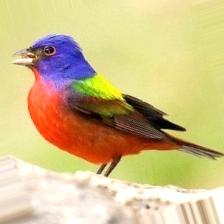
\includegraphics[width=0.24\textwidth]{aug1.jpeg}
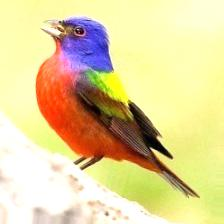
\includegraphics[width=0.24\textwidth]{aug2.jpeg}
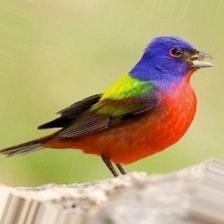
\includegraphics[width=0.24\textwidth]{aug3.jpeg}
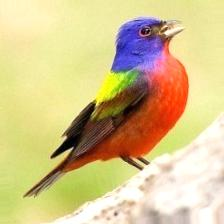
\includegraphics[width=0.24\textwidth]{aug4.jpeg}
	\caption{Rotation, shearing, flipping and brightness adjustments applied to a picture}
\end{figure}




\subsection{Mixup}
The concept of Mixup was introduced by \href{https://arxiv.org/pdf/1710.09412.pdf}{Zhang et al}(2018) and is really fascinating because of its' creativeness and ability to improve performance while being very simple. 

Mixup is a data augmentation teqnique which creates virtual training example by combining two images by 

\begin{align*}
&\tilde{x} = \lambda x_i + (1-\lambda) x_j, \qquad \text{where $x_i$, $x_j$ are input vectors} \\
&\tilde{y} = \lambda y_i + (1-\lambda) y_j, \qquad \text{where $y_i$, $y_j$ are one-hot endoced labels}
\end{align*}


where $(x_i, y_i)$ and $(x_j, y_j)$ are two randomly drawn examples from the training data, and $\lambda$ 
is a probability, that is $\lambda \in [0,1]$. Some examples where mixup where performed is shown in Figure 1.  Usually, $\lambda$ is randomly drawn from a Beta$(\alpha, \alpha)$ 
distribution, for each pair of images which are to be combined. This distribution seems like a 
reasonable chioce since it has the right support and the Beta-distribution is the most natural distribution to
consider when working with probabilities. The Beta$(\alpha, \alpha)$-distribution is also symmetric around $0.5$, which may be 
a desireable property, however this should not matter since we combine our randomly drawn examples with weights $\lambda$ and $1-\lambda$ and 
it would not matter if, for example $\lambda = 0.2$ or $\lambda = 0.8$ since it would yield the same two weights, but in different order, but 
since our examples are randomly drawn the order of the weight should not have an impact. 

When reading about mixup, the use of the Beta-distribution is usually taken for granted, however, there are many other distribution which 
could be considered since the only requirement is that the distribution satisfy $\lambda \in [0,1]$. We will therfore not only consider the 
Beta-distribution. 

WRITE ABOUT OTHER DISTRIBUTION(S) (logit-normal)

We will also consider only performing mixup on the input vectors of the training images but letting $\tilde{y}$ keep the label of the exemple 
with the highest weight. That is,

\begin{align*}
\tilde{y} = I_{\{ \lambda \leq 0.5 \}} y_i + (1-I_{\{ \lambda \leq 0.5 \}}) y_j, 
\end{align*}

where $I_{\{ \lambda \leq 0.5 \}} = 1$ if $\lambda \leq 0.5$ and $0$ otherwise.



\begin{figure}[!htb]
	\minipage{0.32\textwidth}
	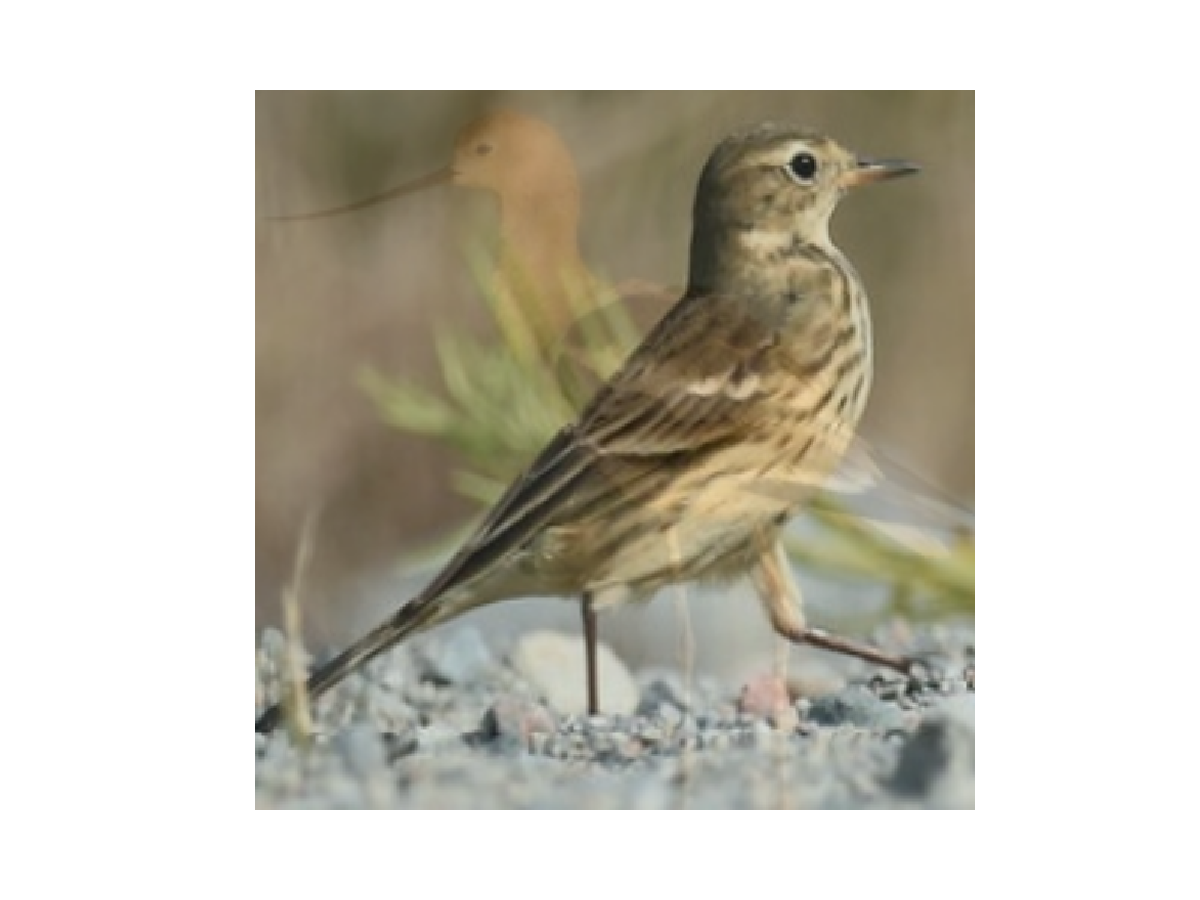
\includegraphics[trim=3cm 2cm 3cm 3cm, width=\linewidth]{mixup1.pdf}
	\endminipage\hfill
	\minipage{0.32\textwidth}
	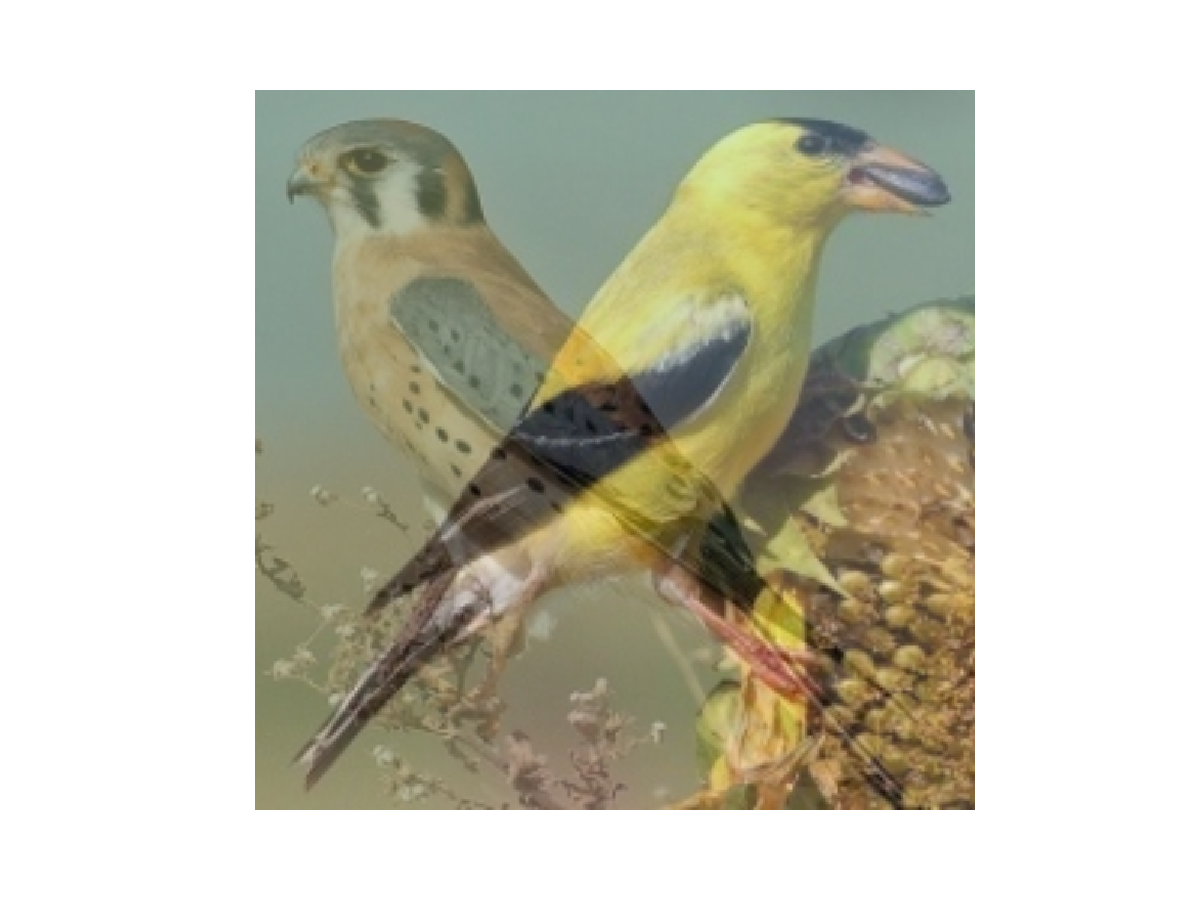
\includegraphics[trim=3cm 2cm 3cm 3cm, width=\linewidth]{mixup2.pdf}
	\endminipage\hfill
	\minipage{0.32\textwidth}%
	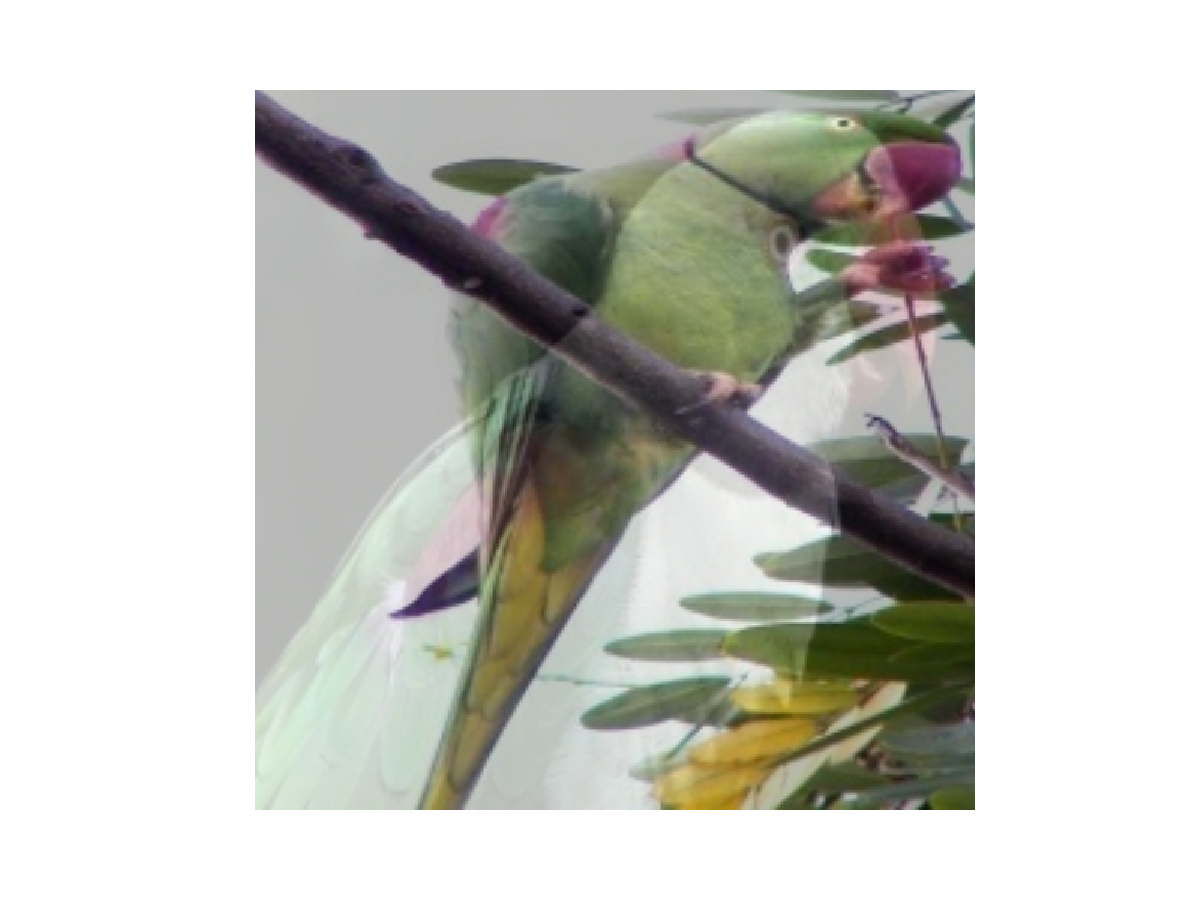
\includegraphics[trim=3cm 2cm 3cm 3cm, width=\linewidth]{mixup3.pdf}
	\endminipage
	\caption{Three examples of mixup performed om images of different bird species.}
\end{figure}

\subsection{Fourier Transformation}

The 2D Fourier transform is used in for instance in image compression and gave us the idea of the possibility using it in deep learning and image classification. 
The 2D fast Fourier transform take our image, with size $[224 \times 224 \times 3]$, as input and return a complex matrix of the same size. From this output we can now get the amplitudes 
by taking the absolute value of each element in the matrix and the phase angles by computing $arctan(y, x)$, where $x$ is the real part and $y$ is the complex part. 
An interesting property is that the phase angels are more important than the amplitudes and contain more information necessary to recreate the image again. 
As an example, in Figure 2 the Fourier transform was applied to two images which yielded amplitudes and phase angles respectively. 
The images were then recreated using the amplitudes from the first image and the phase angles from the second image and vise versa. 

\begin{figure}[!htb]
	\centering
	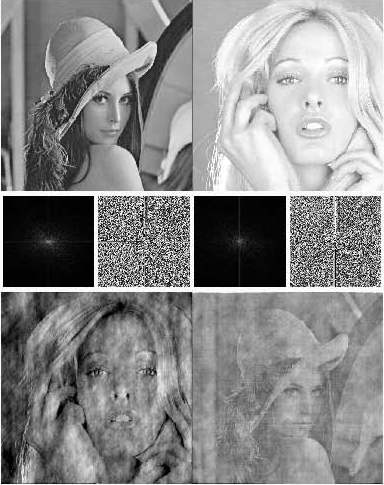
\includegraphics[scale = 0.25]{fourier.jpg}
	\caption{Example of recreation of images using amplitudes and phase angles of the Fourier transformation. 
	Bottom left image use the amplitudes from the first image and the phase angels from the second image and 
	bottom left image use the phase angles from the first image and the amplitudes from the second image}
\end{figure}


Using this as the inspiration we wanted to see if it is true that the phase angles contain more essential information about the image by image classification on the amplitudes 
and phase angels respectively to see if our hypothesis of higher accuracy on the phase angles is satisfied or not. 

Initially we had no expectations that using the fourier transform as augmentation would yield an increase the classification accuracy compared to using 
the raw data, however we thougt it would be an interesting experiment. 
In Figure 3 we can see an example of the Fourier transformation on one of the images in our dataset. 

\begin{figure}[!htb]
	\minipage{0.4\textwidth}
	\raggedleft
	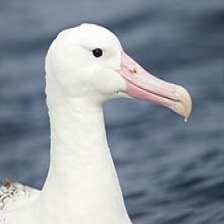
\includegraphics[scale=0.30]{fourier1}
	\endminipage
	\minipage{0.32\textwidth}
	\raggedleft
	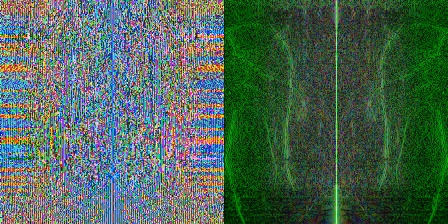
\includegraphics[trim=0cm 0cm 0cm 0cm, scale=0.30]{fourier2}
	\endminipage
	\caption{Left: Original image. Middle: Phase angles. Right: Amplitudes.}
\end{figure}


\section{Experiments}

1.5-2.5 pages

\textit{Discuss the experiments that you performed todemonstrate  that  your  approach  solves  the  problem.   The  exact  ex-periments will vary depending on the project, but you might comparewith previously published methods, perform an ablation study to de-termine the impact of various components of your system, experimentwith different hyperparameters or architectural choices, use visualiza-tion  techniques  to  gain  insight  into  how  your  model  works,  discuss common failure modes of your model, etc.  You should include graphs,tables, or other figures to illustrate your experimental results.}

\subsection{Underlying CNN}

In order to examine the effects of our data augmentation methods we wanted to observe them for a variety of networks with different baseline performances. We used both transfer as well as deep learning in order to examine the data augmentation techniques. Below are the networks we examined and roughly their baseline, i.e. without any augmentation, accuracy on the birds dataset after some training.

\begin{enumerate}[(i)]
 \item Basic CNN (65\%)
 \item MobileNet trained on ImageNet (75\%)
 \item ResNet50 trained on ImageNet (95\%)
\end{enumerate}

\begin{figure}[h]
	\centering
	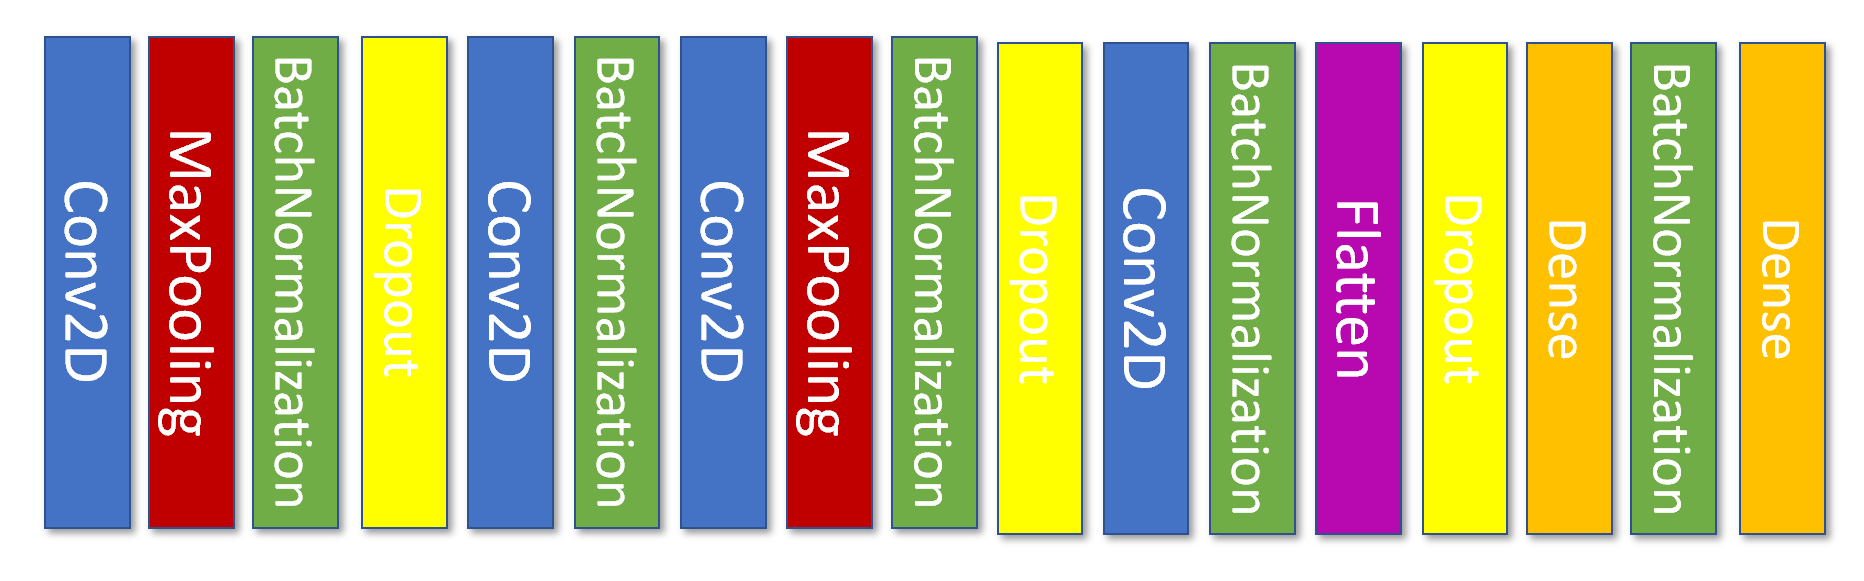
\includegraphics[width=0.9\textwidth]{conv.PNG}
	\caption{Layers of the basic CNN}
\end{figure}

\subsection{Augmentations}

\subsubsection{The Fourier Transform}

In order to ascertain what components of the fourier transform, that is the angles, the amplitudes or the combination of them, which generated the best results we examined their respective performances using the basic CNN architechture. The network was trained for 20 epochs in each experiment using a batch size of 100 and a learning rate of 0.01 in combination with momentum and some decay. It should be noted that the training time increases drastically when taking both the angles and the amplitudes into account as the dimensions of the input increases.

\begin{table}[H]
  \caption{Basic CNN}
  \label{sample-table}
  \centering
  \begin{tabular}{ll}
    \toprule
    Data & Accuracy (\%) \\
    \midrule
    Raw Images  & 64.59 \\
    Fourier Angles & 28.84   \\
    Fourier Amplitudes & 48.42 \\
    Fourier Angles \& Amplitueds & 47.42 \\
    \bottomrule
  \end{tabular}
\end{table}

For the basic CNN it seems as if using only the amplitudes generated the highest accuracy which seems to contradict what we initially thought about the phase angles containing more information about the content of the image. In all it seems as if the Fourier transform of the input data is not a valid method in order to improve the performance of a CNN, or at least not in the case of our bird data. An interesting extension could be to apply this method to different datasets with more internal variety, such as for example CIFAR-100. 

\medskip

Due to computational constraints as well as the quite clear results from the performance on the Basic CNN we did not evaluate the effects of the Fourier Transform on either MobileNet or ResNet50. A major reason for this is that the pre-trained weights from ImageNet are in no way compatible with our angles and amplitudes which would imply a complete re-training using the base architechtures.

\section{Conclusions}

0.25-0.5 pages

\textit{Summarize your key results - what have you learned? Suggest ideas for future extensions or new applications of your ideas.}

What we have implemented is \textit{input mixup} where we do all augmentation before training and input the images in the network after performing mixup, however https://arxiv.org/pdf/1806.05236.pdf 
suggest a new algorithm called \textit{manifold mixup} where mixup is performed at an intermediate layer or final layer in the network. In an intermediate layer 
the feature spaces are more aligned than that of the input and it is suggested that mixup will produce better augmented data if the mixup is performed on this layer. Therefore, this would be 
a natural possible future extention to this project. 


\section*{References}

Exempel:
\medskip

\small

[1] Alexander, J.A.\ \& Mozer, M.C.\ (1995) Template-based algorithms for
connectionist rule extraction. In G.\ Tesauro, D.S.\ Touretzky and T.K.\ Leen
(eds.), {\it Advances in Neural Information Processing Systems 7},
pp.\ 609--616. Cambridge, MA: MIT Press.

\section{info (ska ej vara med i rapporten)}

-Total 6-8 sidor inkl referenser och appendix


\end{document}
